% TEXINPUTS=.:$HOME/git/bvtex: latexmk  -pdf <main>.tex
\documentclass[xcolor=dvipsnames]{beamer}

\input{defaults}
\input{beamer/preamble}

\setbeamertemplate{navigation symbols}{}
% \setbeamertemplate{background}[grid][step=1cm]

\usepackage{siunitx}
\usepackage{xmpmulti}
\usepackage[export]{adjustbox}

\usepackage[outline]{contour}
\usepackage{tikz}
\usetikzlibrary{shapes.geometric, arrows}
\usetikzlibrary{positioning}

\definecolor{bvtitlecolor}{rgb}{0.98, 0.92, 0.84}
\definecolor{bvoutline}{rgb}{0.1, 0.1, 0.1}

\renewcommand{\bvtitleauthor}{Brett Viren\\\small for the BNL Wire Cell Group}
\renewcommand{\bvtit}{Wire Cell}
\renewcommand{\bvtitle}{\LARGE Wire Cell Reconstruction Method and Software Library\\\Large for Liquid Argon Time Projection Chambers}
\renewcommand{\bvevent}{\textbf{Connecting The Dots 2016}}
\renewcommand{\bvbeamerbackground}{}

% http://tex.stackexchange.com/a/23550
\makeatletter
\providecommand{\beamer@slideinframe}{0}%
\tikzset{highlight/.code={\ifnum#1=\beamer@slideinframe \tikzset{draw=red,text=red}\fi},highlight/.value required}
\makeatother

\setbeamertemplate{headline}{%
\leavevmode%
  \hbox{%
    \begin{beamercolorbox}[wd=\paperwidth,ht=2.5ex,dp=1.125ex]{palette quaternary}%
    \insertsectionnavigationhorizontal{\paperwidth}{}{\hskip0pt plus1filll}
    \end{beamercolorbox}%
  }
}
\begin{document}
\input{beamer/title.tex}
\input{beamer/toc.tex}

\lstset{%
  language=C++,
                basicstyle=\scriptsize\ttfamily,
                keywordstyle=\color{blue}\ttfamily,
                stringstyle=\color{red}\ttfamily,
                commentstyle=\color{gray}\ttfamily,
                morecomment=[l][\color{magenta}]{\#}
}

\section {LArTPC Detectors}


\begin{frame}
  \frametitle{LArTPC Experiments - ICARUS}

  The origin of LArTPC technology for Neutrinos: \href{http://cds.cern.ch/record/117852/files/CERN-EP-INT-77-8.pdf}{C. Rubbia, 1977} led to \textbf{ICARUS, the first, large-scale LArTPC}.

  \begin{columns}
    \begin{column}{0.5\textwidth}
      \begin{itemize}
      \item $2\times$ \SI{300}{\tonne} modules.
      \item Took data in the Gran Sasso tunnel, Italy from CERN
        neutrino beam.
      \item Moving to Fermilab as part of the \textbf{Short-Baseline
        Neutrino} Program.
      \end{itemize}
    \end{column}
    \begin{column}{0.5\textwidth}
      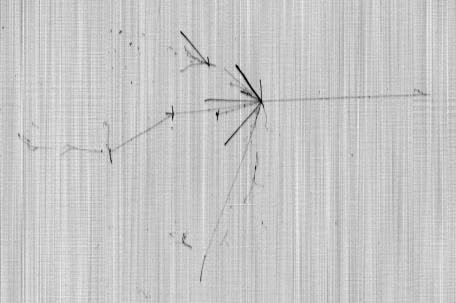
\includegraphics[width=0.8\textwidth]{icarus.png}
    \end{column}
  \end{columns}
\end{frame}

\begin{frame}
  \frametitle{LArTPC Experiments - MicroBooNE}

  \begin{center}
    Recently started taking $\nu$-data at Fermilab!    
  \end{center}

  \begin{columns}
    \begin{column}{0.5\textwidth}
      \begin{center}
        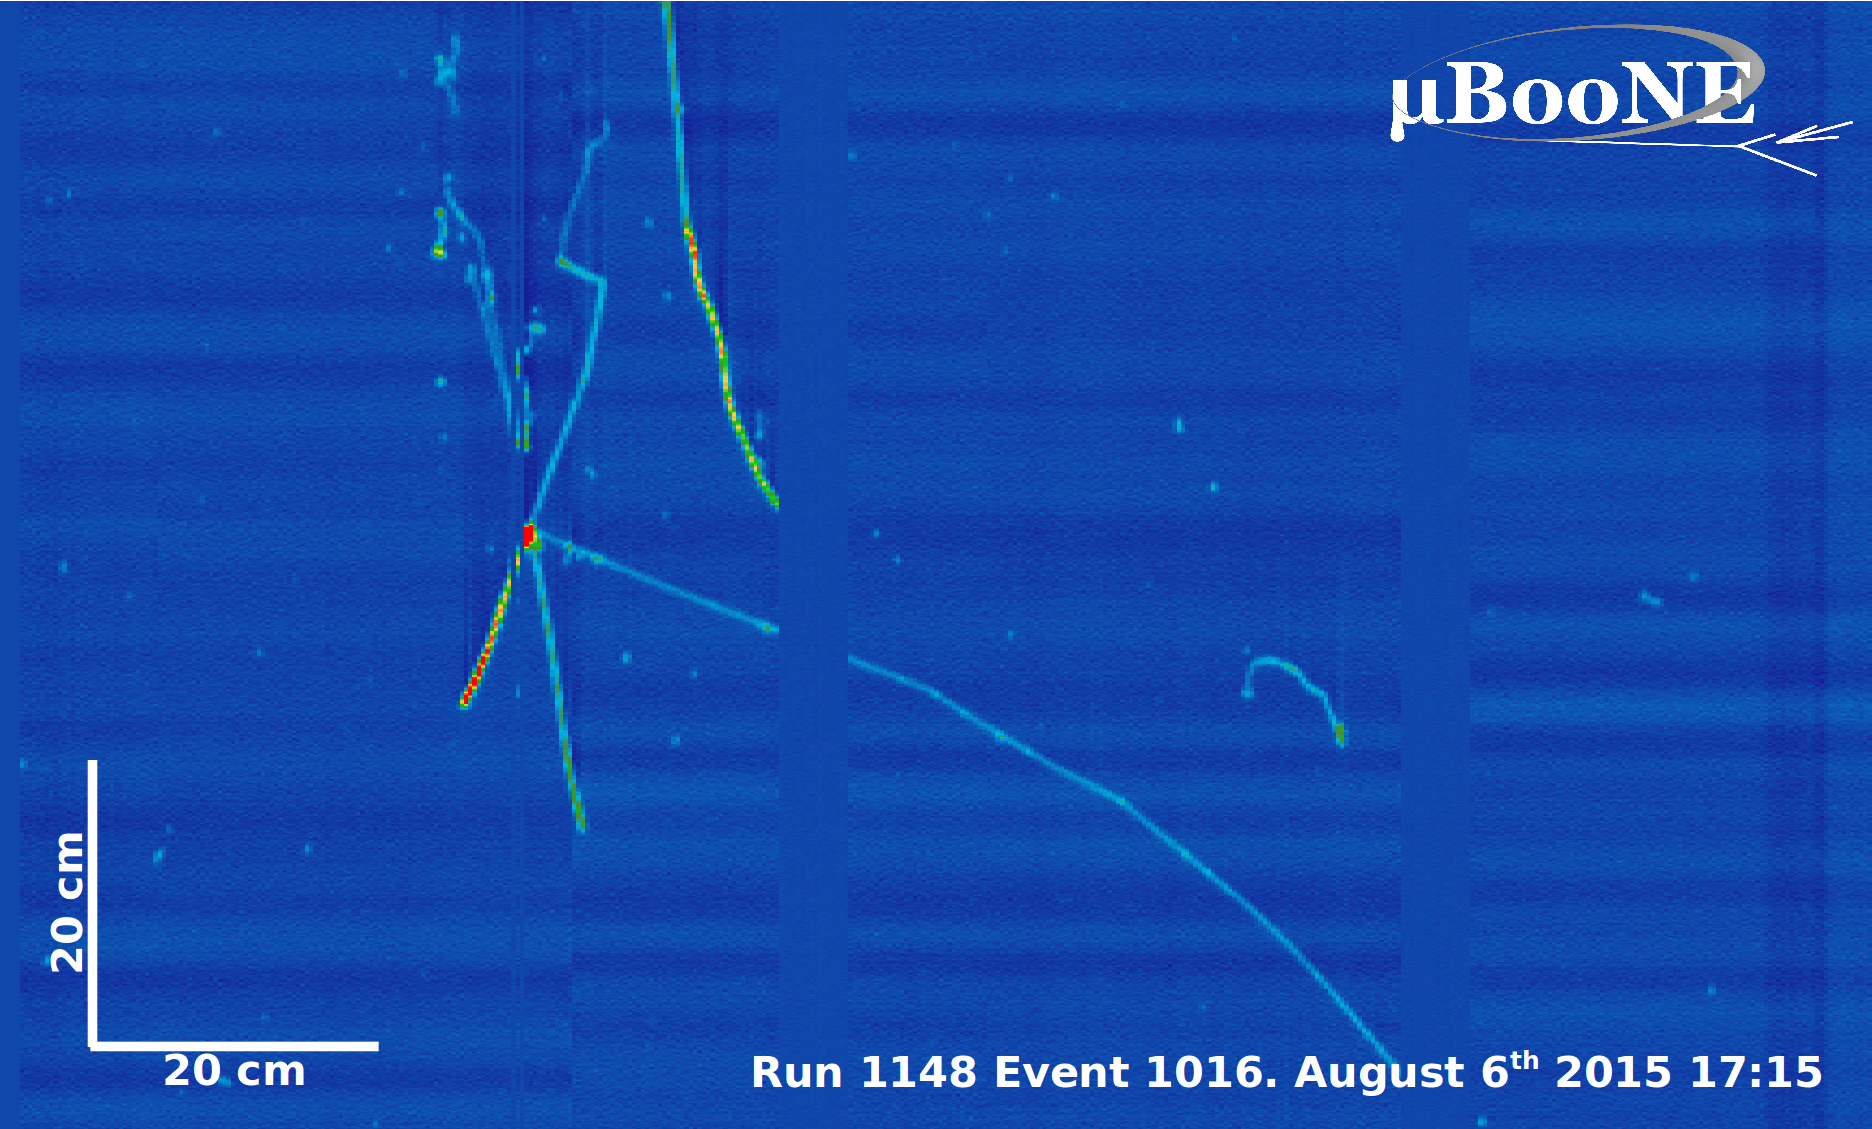
\includegraphics[width=0.9\textwidth]{run1148_ev1016.png}
      \end{center}

    \end{column}
    \begin{column}{0.5\textwidth}
      \begin{itemize}
      \item 85 ton fiducial mass.
      \item 8256 channels
      \item 3 mm wire pitch.
      \item Investigate:
        \begin{itemize}\footnotesize
        \item low energy excess puzzle
        \item sterile-$\nu$ search
        \item $\nu$-Ar cross sections
        \end{itemize}
      \end{itemize}
    \end{column}
  \end{columns}

  \vspace{3mm}

  \begin{center}
    MicroBooNE is the initial test bed for Wire Cell reconstruction.    
  \end{center}

\end{frame}

\begin{frame}[fragile]
  \frametitle{LArTPC Experiments - 
\includegraphics[height=7mm,trim=4cm 9.2cm 4cm 9.3cm,clip,valign=c]{DUNElogo_colorHORIZONTAL.pdf}}
  \begin{center}
    ``International \textbf{mega-science} project''

    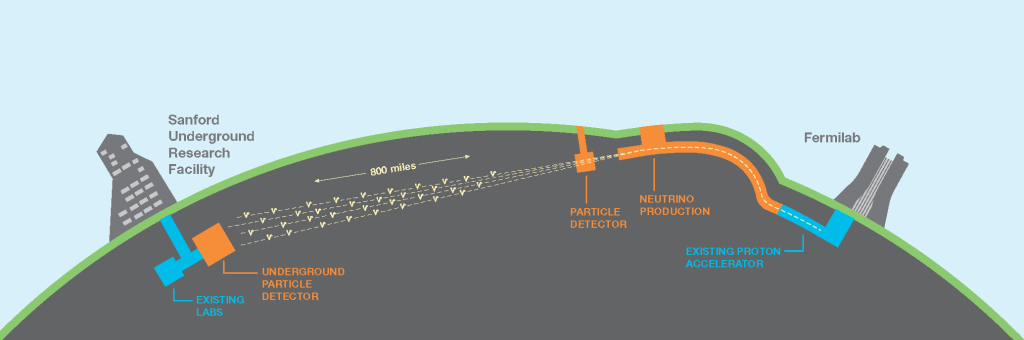
\includegraphics[height=25mm]{LBNF_Graphic_021715-1024x340.png}
  \end{center}


  Three stages of DUNE LArTPC detectors:
  \begin{enumerate}\footnotesize
  \item ``\textbf{35ton}'' prototype (at FNAL), just started operating, cosmic-$\mu$ exposure. 
  \item Full-scale ``\textbf{protoDUNE}'' (at CERN) 2017/2018 with $\pi, K, p$ beam tests.
  \item Full ``\textbf{DUNE}'' far detector underground in South Dakota $\sim$2025.
    \begin{itemize}
    \item At least \textbf{10 kt} of single-phase LAr, 3-plane, wire readout: \\
      5 mm wire pitch, \textbf{375K channels}.

    \item Total of \textbf{40 kt fiducial mass} in \textbf{4 separate cryostats}, \\
      \footnotesize{different technologies possible for each module.}

    \end{itemize}
  \end{enumerate}

\end{frame}

\begin{frame}
  \frametitle{LArTPC with Wire Readout - Basics Principles}

  \begin{itemize}
  \item Charged particles produce tracks of ionized LAr
  \item Electrons drift in an applied electric field 
    \begin{itemize} \footnotesize
    \item Eg: E = \SI{500}{\volt/\cm}, $v_{\mbox{drift}}=$ \SI{1.6}{\milli\meter/\micro\second}
    \end{itemize}
  \item Charge drifts past 3 parallel wire planes (\num{3}-\SI{5}{\milli\meter} pitch)
    \begin{itemize}
    \item 2 induction planes with bipolar signals.
    \item 1 collection plane with monopolar signals.
    \end{itemize}
  \item Digitize wire signal waveforms (\SI{2}{\mega\hertz}, 12 bits)
  \item Deconvolve detector response and apply noise filter.
  \item Optical system gives prompt $T_0$ from scintillation light.
  \end{itemize}

  \begin{itemize}
  \item [$\rightarrow$] Gives \textbf{three independent measures} of
    each element of drifting charge as \textbf{three, 2D views} (in \textbf{wire
    vs time}) which \textbf{multiplex the two transverse dimensions}.
  \end{itemize}

  \vfill

  \flushright\footnotesize{(animation by Bo Yu $\rightarrow$)}

\end{frame}

\begin{frame}[fragile]
  \begin{center}
      \multiinclude[<+->][format=png, graphics={trim=0cm 1.6cm 0cm 2cm, clip,height=0.9\textheight}]{signal}
  \end{center}
\end{frame}

\begin{frame}
  \frametitle{LArTPC Data}
  
  \vspace{-10mm}

  \begin{columns}
    \begin{column}{0.8\textwidth}
      LArTPC can produce \textbf{huge quantities} of \textbf{high-resolution} data from \textbf{large detector volumes}:
      \begin{itemize}
      \item $10^4$ -- $10^6$ channels
      \item 2MHz @ 12 bit waveform digitization
      \item each ``event'' spans several milliseconds
      \end{itemize}
    \end{column}
    \begin{column}{0.2\textwidth}
      \begin{center}
        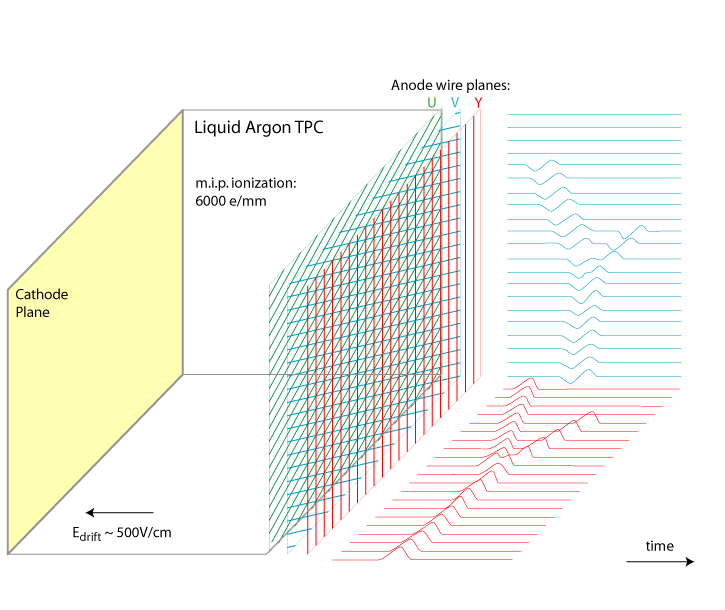
\includegraphics[width=\textwidth,trim=13cm 0cm 0cm 0cm,clip]{signal-15.png}

        %\scriptsize \SI{0.5}{\micro\second} waveform digitization.
      \end{center}
    \end{column}
  \end{columns}

  \vspace{-5mm}

  \footnotesize
  Two general DAQ readout strategies:
  \begin{description}
  \item[Full Stream:] read out entire waveform (\textbf{MicroBooNE})
    \begin{itemize}
    \item \textbf{30GB/s in 120 MB ``events''}.
    \item DUNE at FS would produce 5 TB/s in 25 GB ``events''!
    \end{itemize}
  \item[Zero Supression:] only save waveform parts with significant activity (\textbf{DUNE})
    \begin{itemize}
    \item Threshold chosen based on noise ($E_{thesh} \sim$\SI{0.1}{\mega\electronvolt}/wire)
    \item 2.5 MB/event $\rightarrow$ \textbf{100's TB/year}
    \item requires rejection of natural $^{39}$Ar decay @ \textbf{50 PB/year}
    \end{itemize}
  \end{description}

\end{frame}


\section{Technique}

\begin{frame}
  \tableofcontents[currentsection,hideothersubsections]
\end{frame}


\begin{frame}[fragile]
  \frametitle{Wire Cell Reconstruction Method}
  \setbeamercovered{transparent}
  \begin{columns}
    \begin{column}{0.7\textwidth}
      Four main parts:
      \begin{enumerate}
      \item<2> Data Preparation
        \begin{itemize}        \scriptsize
        \item Deconvolve \textbf{detector response and filter noise}.
        \item Construct \textbf{wire} geometry and associated \textbf{cells}.
        \item Read framed data stream, form \textbf{time slices}
        \end{itemize}
      \item<3> Imaging of Activity
        \begin{itemize}        \scriptsize
        \item The heart of the Wire Cell technique
        \item Identify the likely hit \textbf{cells} in each time slice.
        \end{itemize}
      \item<4> Pattern Recognition 
        \begin{itemize}         \scriptsize
        \item Application of Wire Cell imaging
        \item \textbf{Cluster} activity in space and across time slices.
        \item \textbf{Categorize}: track, shower, etc.
        \end{itemize}
      \item<5> Physics Quantities
        \begin{itemize}         \scriptsize
        \item Determine particle ID and kinematics of tracks/showers.
        \end{itemize}
      \end{enumerate}
    \end{column}
    \begin{column}{0.3\textwidth}
      \begin{center}
        \vspace{-10mm}
        \resizebox{!}{\textheight}{
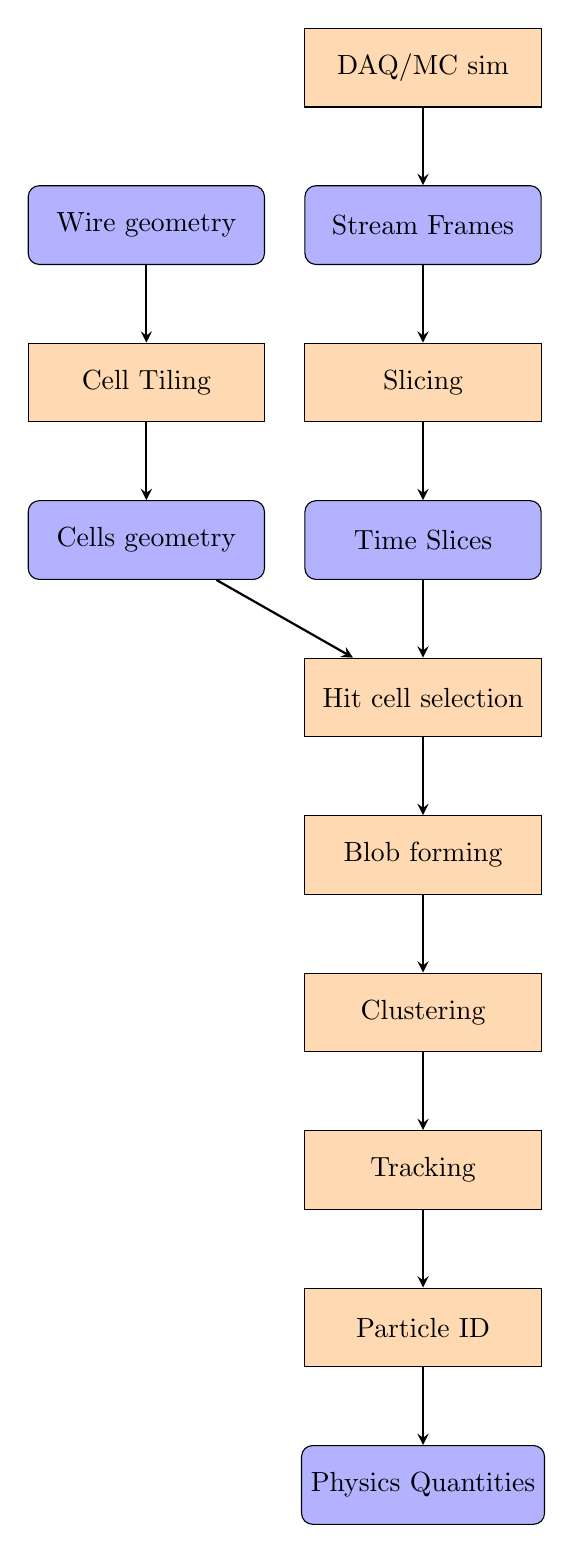
\begin{tikzpicture}[align=center, node distance=2cm]

\tikzstyle{dataobj} = [rectangle, rounded corners, minimum width=3cm, minimum height=1cm,text centered, draw=black, fill=blue!30]
\tikzstyle{process} = [rectangle, minimum width=3cm, minimum height=1cm, text centered, draw=black, fill=orange!30]
\tikzstyle{decision} = [diamond, minimum width=3cm, minimum height=1cm, text centered, draw=black, fill=green!30]
\tikzstyle{arrow} = [thick,->,>=stealth]

\node (daqmc) [process,highlight=2] {DAQ/MC sim};
\node (frames) [dataobj, below of=daqmc] {Stream Frames};
\node (slicing) [process,highlight=2, below of=frames] {Slicing};
\node (slices) [dataobj, below of=slicing] {Time Slices};
\node (wires) [dataobj, left=0.5cm of frames] {Wire geometry};
\node (tiling) [process,highlight=2, left=0.5cm of slicing] {Cell Tiling};
\node (cells) [dataobj, left=0.5cm of slices] {Cells geometry};
\node (hitcells) [process,highlight=3, below of=slices] {Hit cell selection};
\node (blobbing) [process,highlight=3, below of=hitcells] {Blob forming};
\node (clustering) [process,highlight=4, below of=blobbing] {Clustering};
\node (tracking) [process,highlight=4, below of=clustering] {Tracking};
\node (pid) [process,highlight=5, below of=tracking] {Particle ID};
\node (physics) [dataobj, below of=pid] {Physics Quantities};

\draw [arrow] (wires) -- (tiling);
\draw [arrow] (tiling) -- (cells);
\draw [arrow] (cells) -- (hitcells);
\draw [arrow] (daqmc) -- (frames);
\draw [arrow] (frames) -- (slicing);
\draw [arrow] (slicing) -- (slices);
\draw [arrow] (slices) -- (hitcells);
\draw [arrow] (hitcells) -- (blobbing);
\draw [arrow] (blobbing) -- (clustering);
\draw [arrow] (clustering) -- (tracking);
\draw [arrow] (tracking) -- (pid);
\draw [arrow] (pid) -- (physics);
\end{tikzpicture}}
      \end{center}
    \end{column}
  \end{columns}

\end{frame}

\subsection{Data Preparation}


\begin{frame}[fragile]
  \frametitle{Time Slicing}
  
  \begin{columns}
    \begin{column}{0.35\textwidth}
      \begin{center}
        \vspace{-.5cm}

        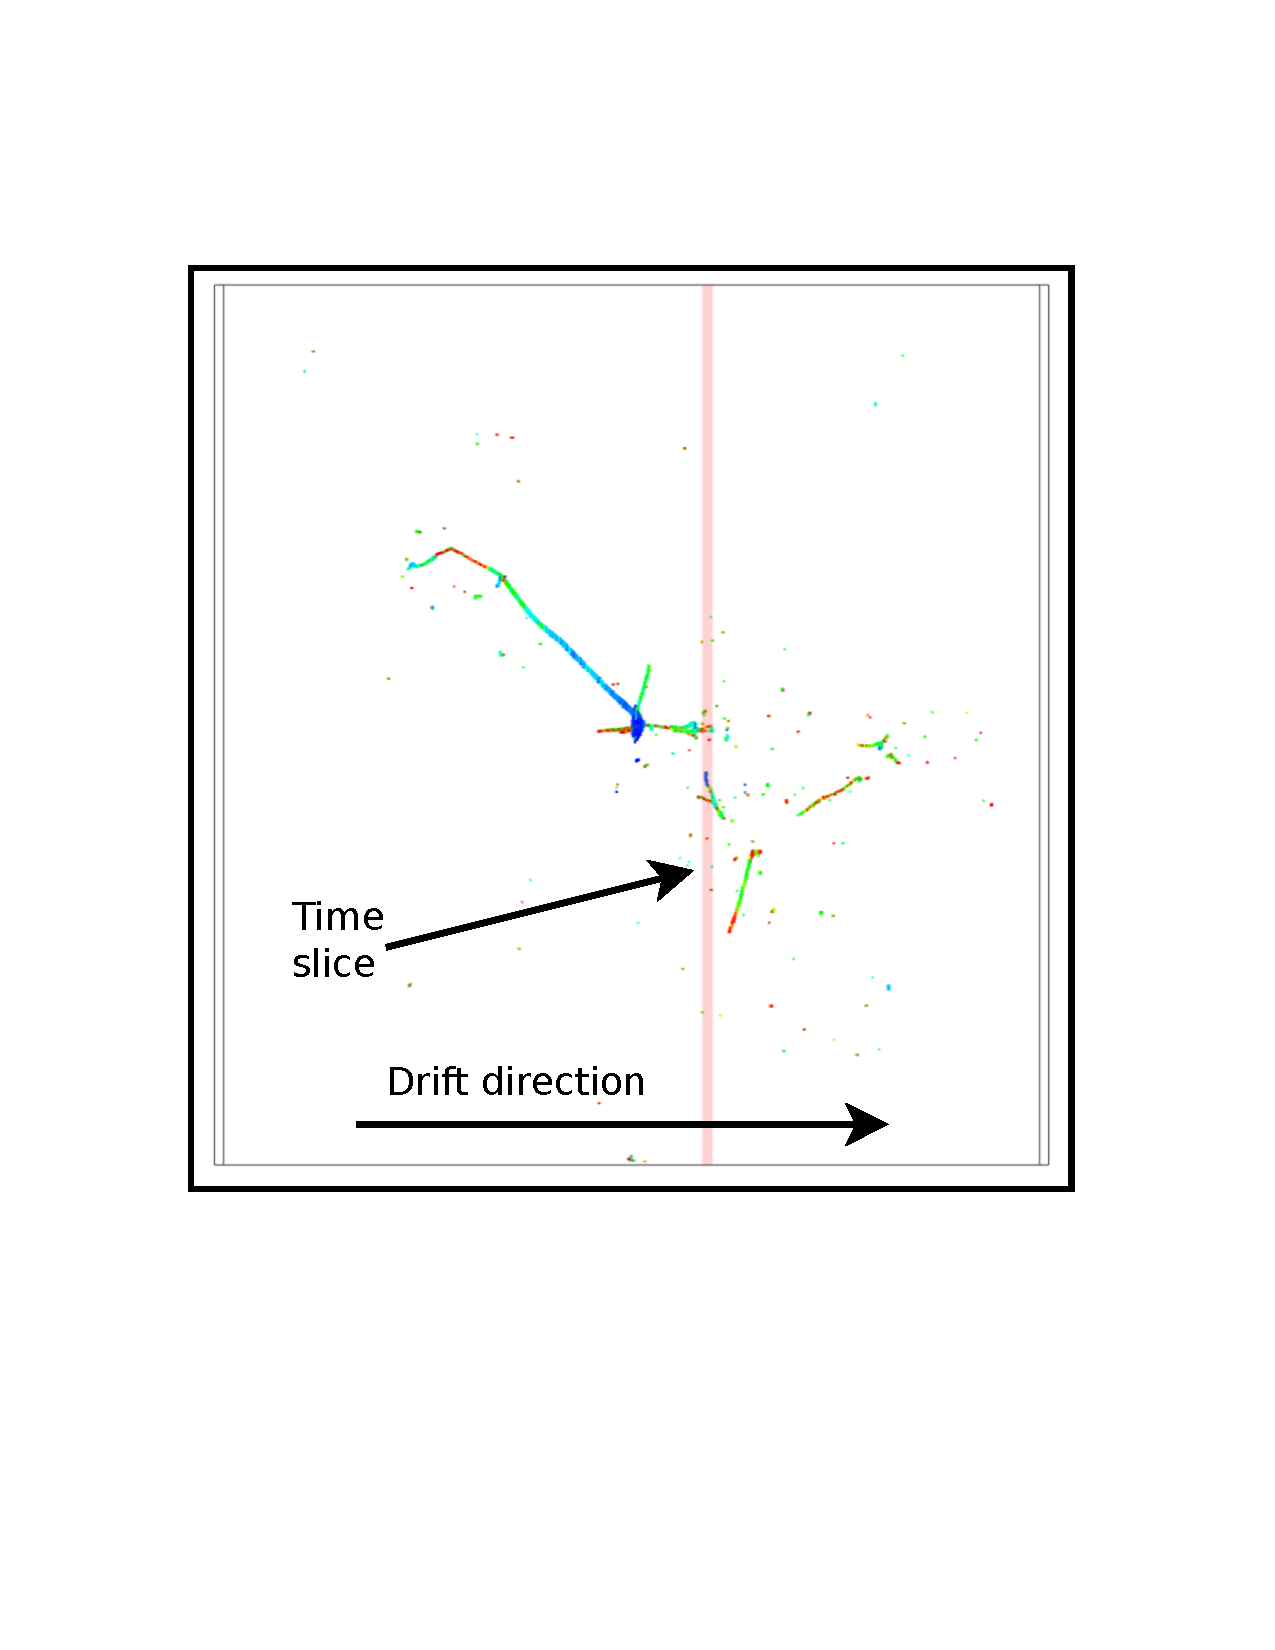
\includegraphics[width=\textwidth]{slice.pdf}

        \vspace{-2cm}

        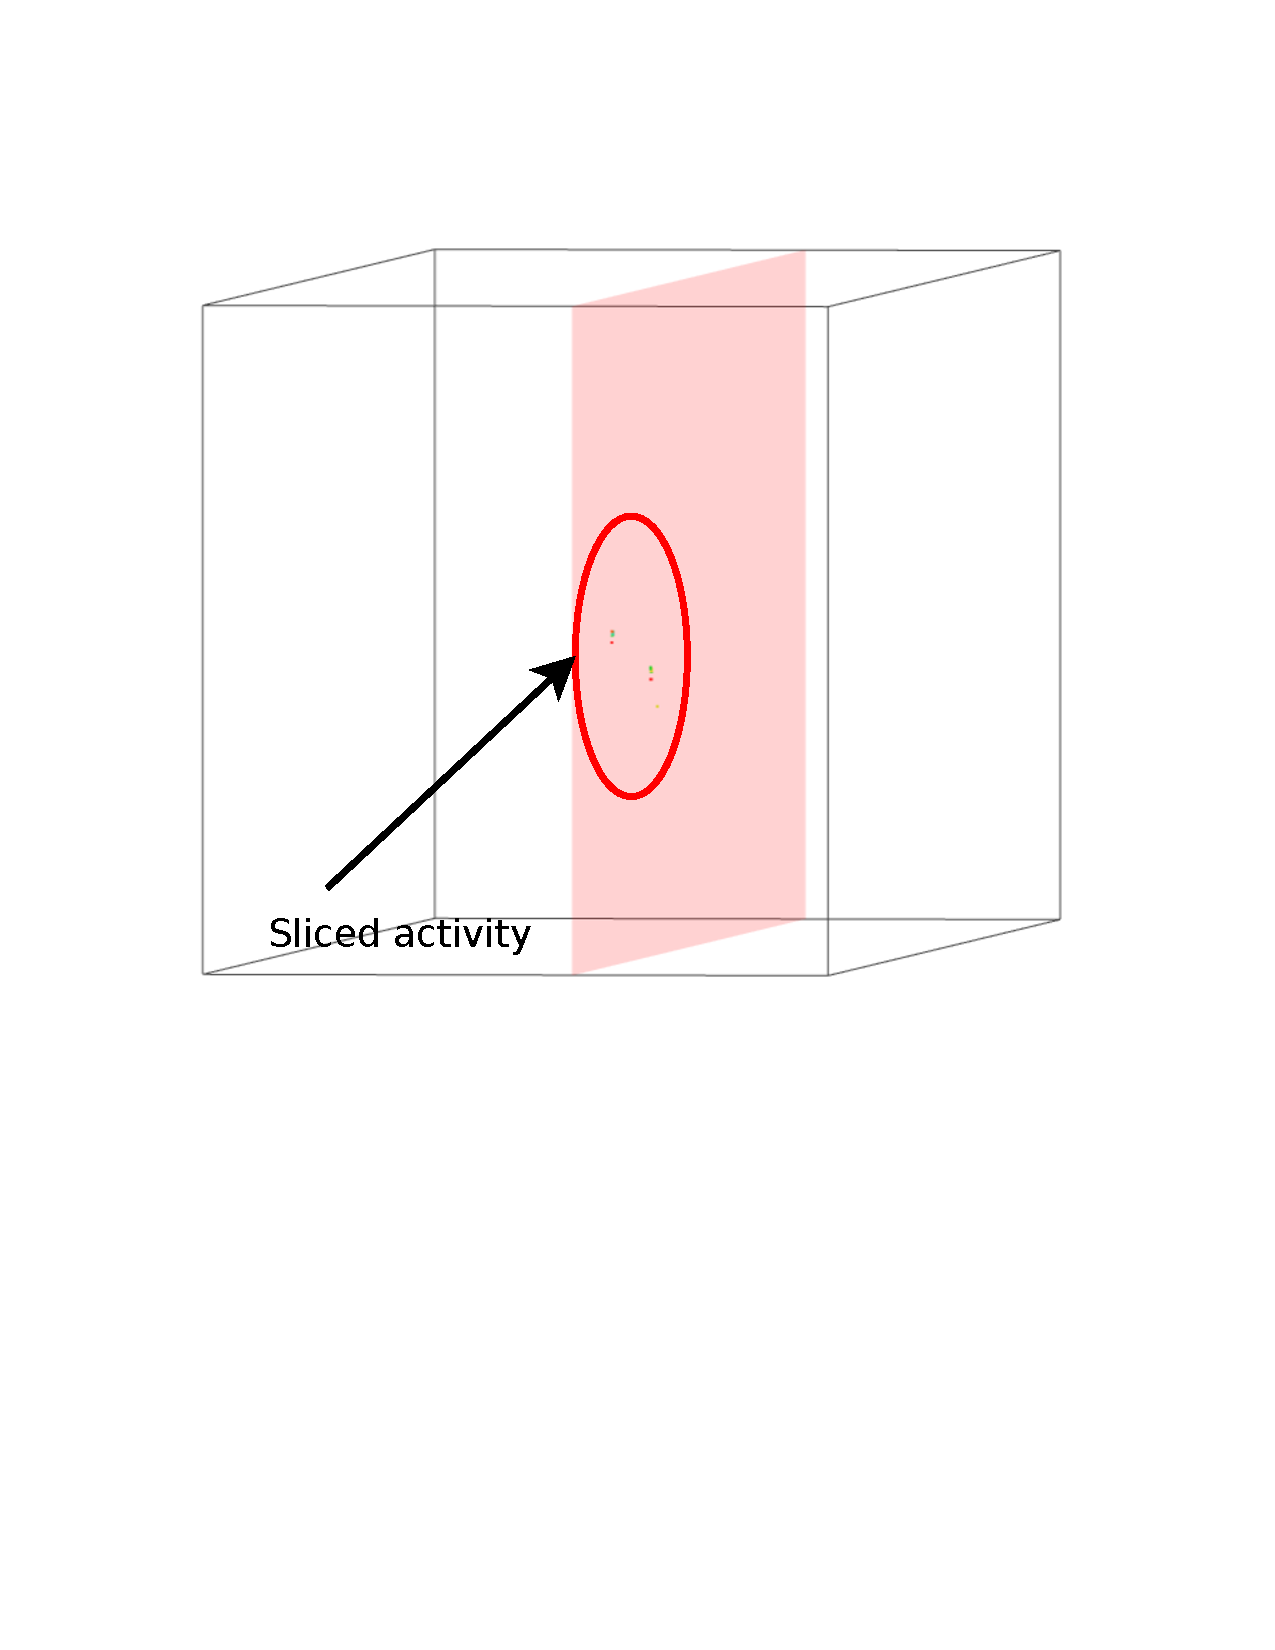
\includegraphics[width=\textwidth,trim=0cm 10cm 0cm 0cm,clip]{slice-3D.pdf}

        \scriptsize Focus on one \textbf{time slice} along a plane transverse to the drift.
      \end{center}
    \end{column}
    \begin{column}{0.65\textwidth}

      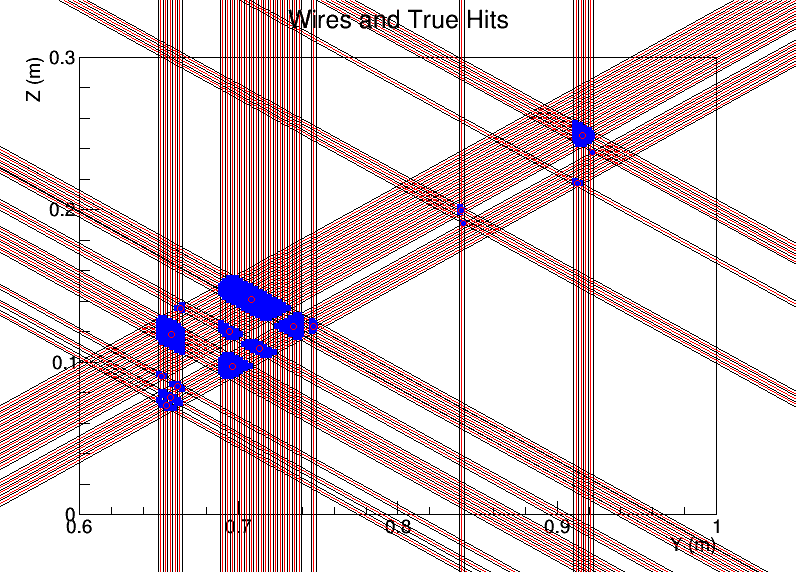
\includegraphics[width=0.9\textwidth]{wires-and-true-hits.png}

      \begin{itemize} \scriptsize
      \item Slice duration is chosen to \textbf{match
          electronics shaping time}: combine 4 FADC ``ticks'' =
        \SI{2}{\micro\second}.
      \item Select \textcolor{red}{wires} above threshold in the slice.
      \item Regions of triple-wire overlap: potential ``\textcolor{blue}{cells}'' holding charge in the \textbf{time slice}.
      \end{itemize}
    \end{column}
  \end{columns}

\end{frame}

\subsection{Imaging Of Activity}

\begin{frame}[fragile]
  \frametitle{Tiling}

  \vspace{-10mm}

  \begin{center}
    \scriptsize Zoom in on the wires and their associated (constructed) cells.

    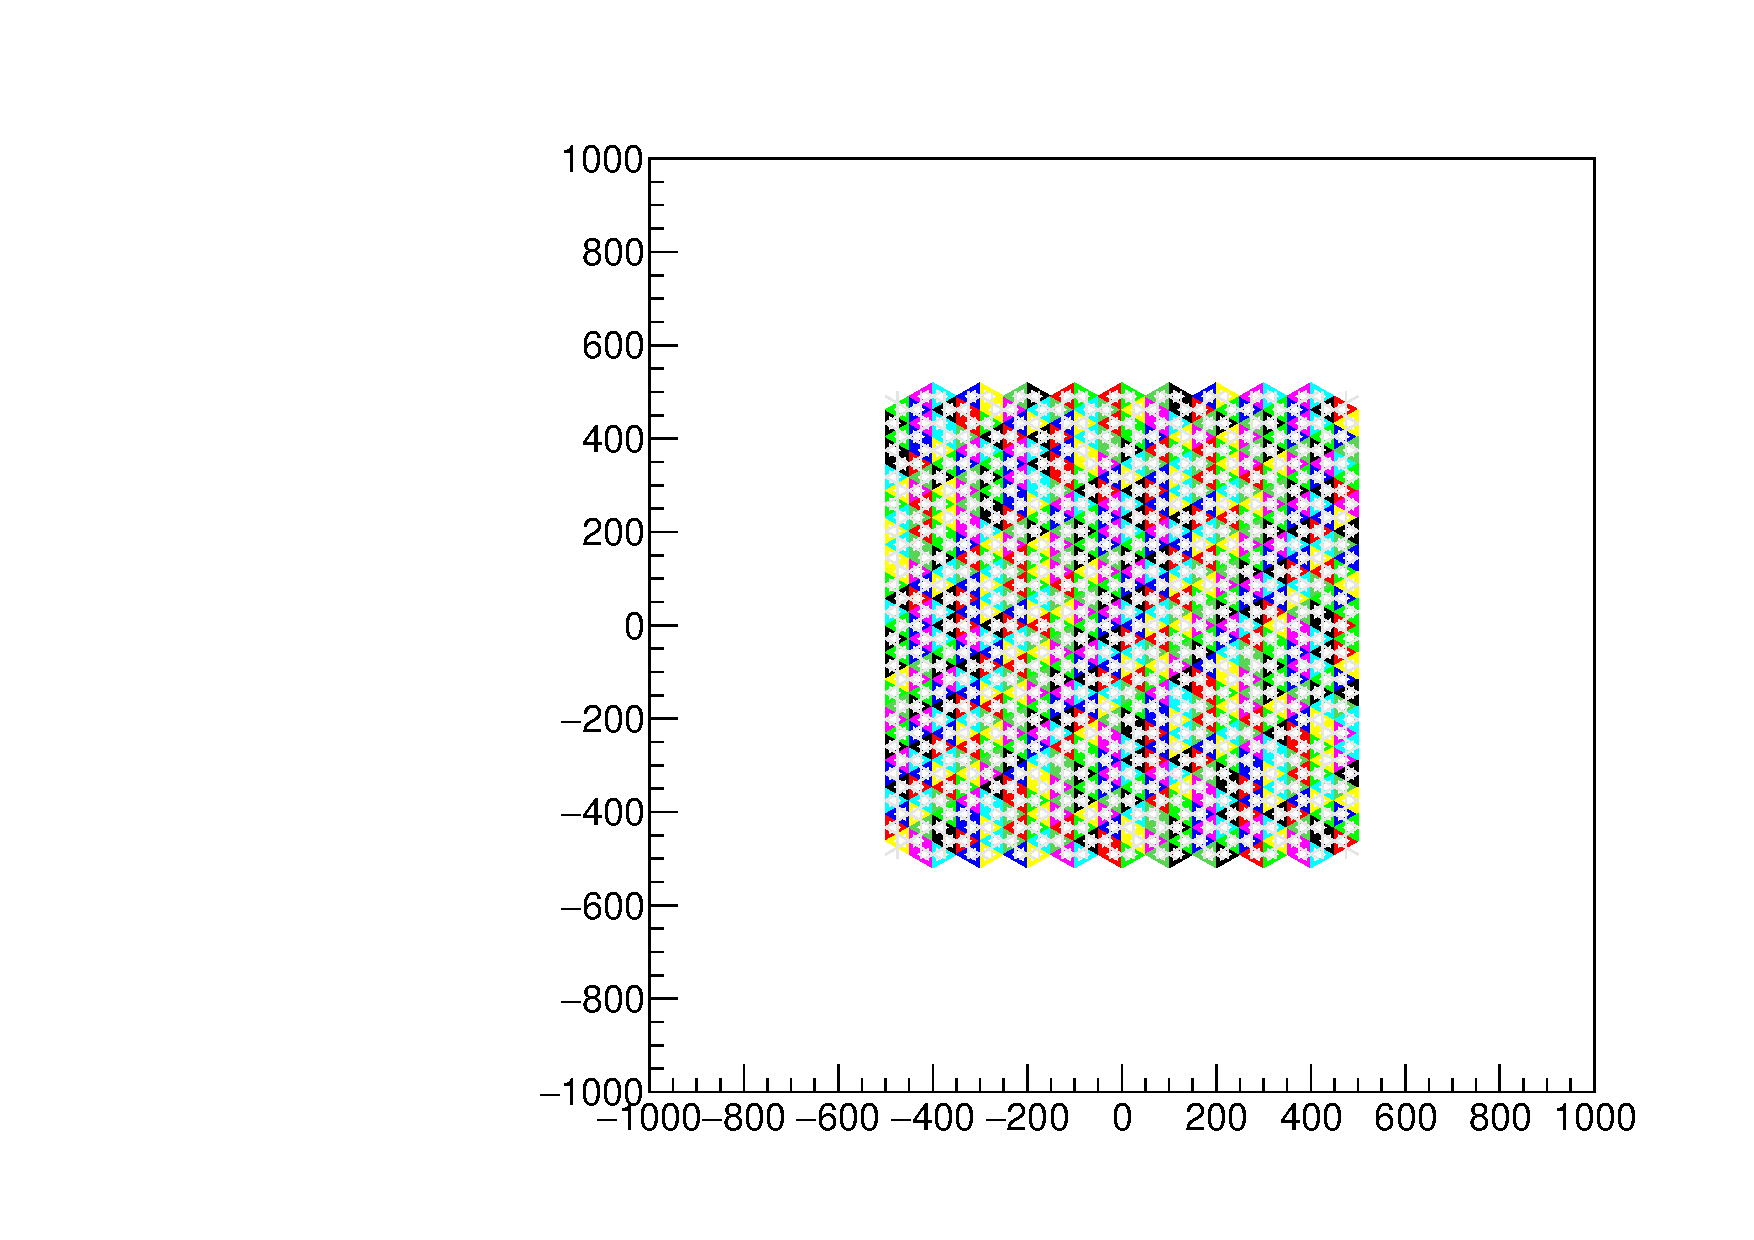
\includegraphics[width=0.7\textwidth,trim=8.6cm 10cm 8.6cm 9cm,clip]{test_boundcells_uboone.pdf}

    MicroBooNE geometry, grey wires, colored cells.
  \end{center}

  \footnotesize
  Cell construction:
  \begin{itemize}
  \item Each ``cell'' a 2D region near \textit{approximate triple crossings} of one wire from each of the three planes.
  \item Cells completely tile the plane.
  \item Cell pattern determined by wire \textbf{pitch}, \textbf{angle} and \textbf{phase}.
    \begin{description}
    \item[MicroBooNE] regular isosceles triangles.
    \item[DUNE] variety of polygons with a spectrum of sizes
    \end{description}
  \end{itemize}

  \textbf{The heart of the Wire Cell concept:} if all three of the
  triple-crossing \textbf{wires} are above threshold in a \textbf{time
    slice}, the associated \textbf{cell} likely contains the element
  of \textbf{drifted charge}.

\end{frame}

\begin{frame}
  \frametitle{Cell Ambiguity - Example Hit Pattern}

  \begin{columns}
    \begin{column}{0.35\textwidth}
      \begin{center}
        \scriptsize Zoom in on $5 \times 5 \times 3$ wires:

        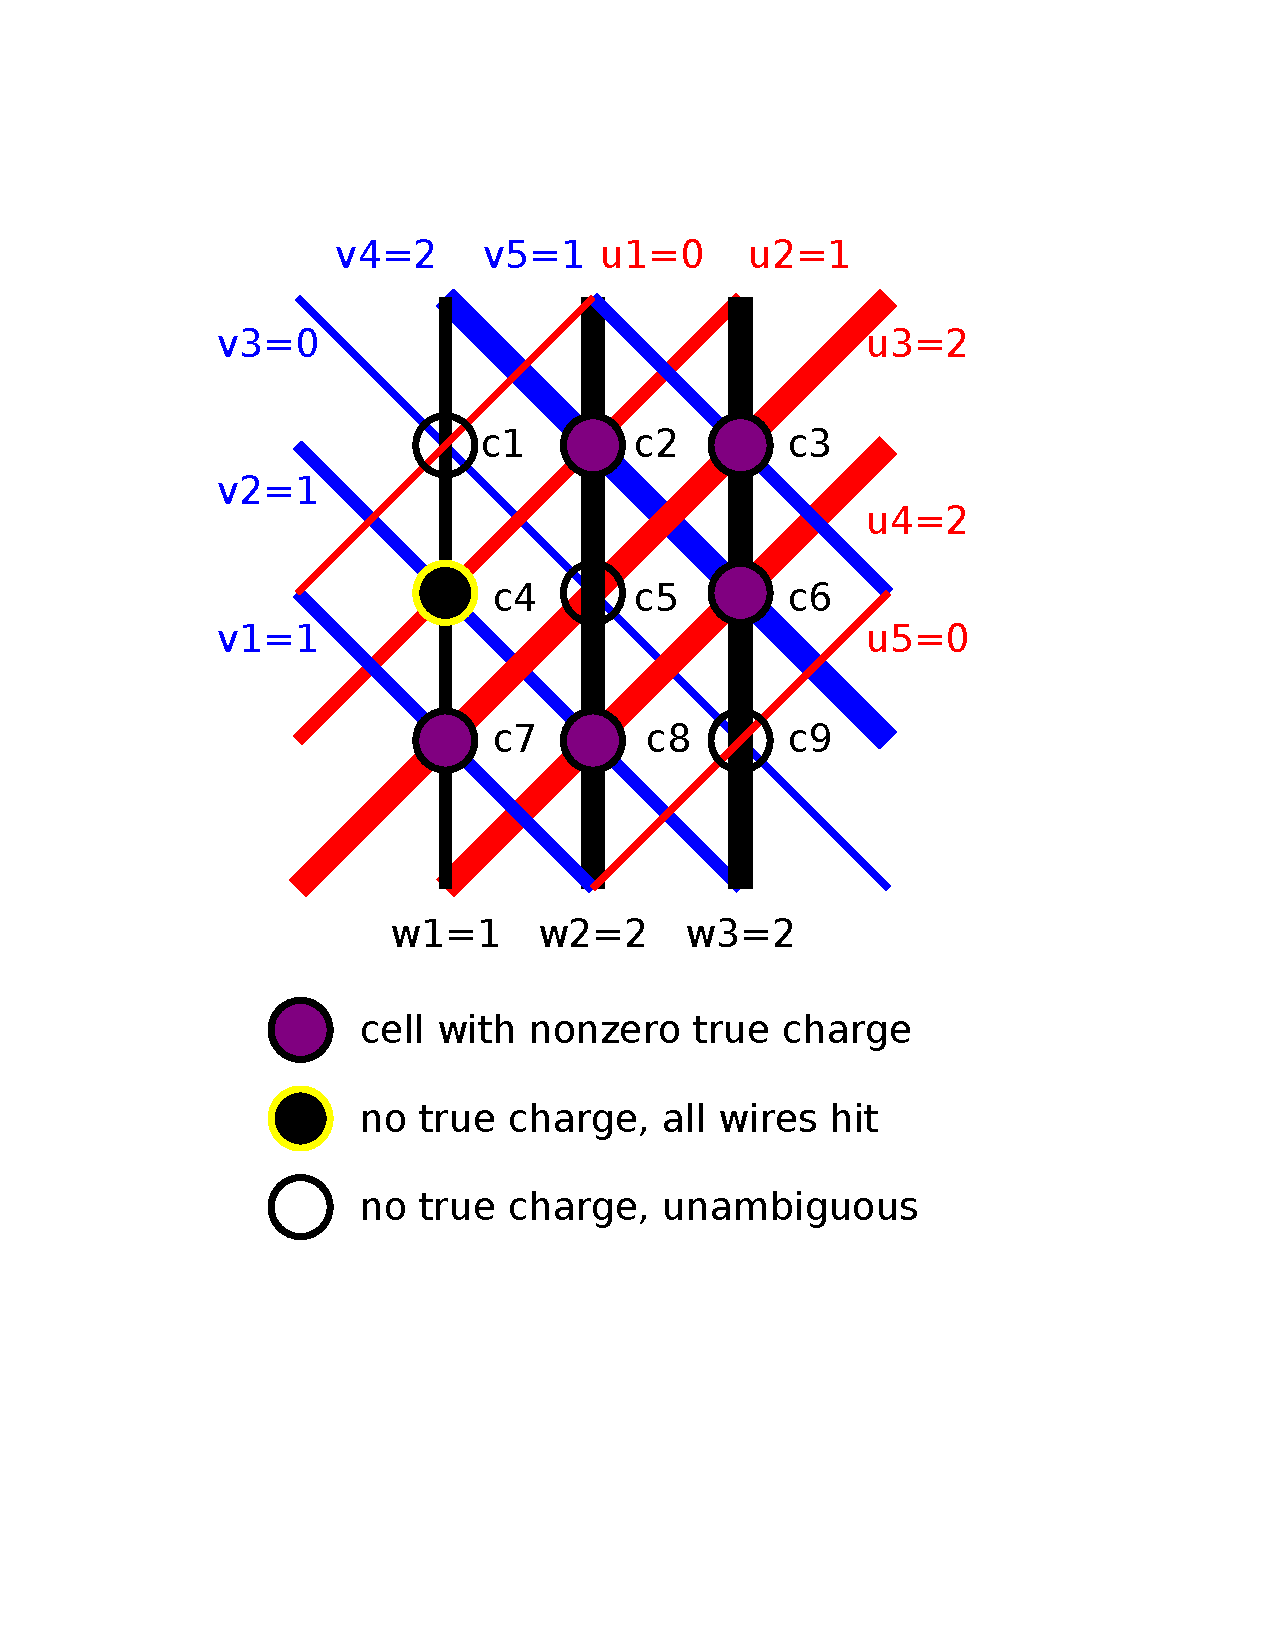
\includegraphics[width=\textwidth,trim=3.5cm 6cm 5cm 3cm,clip]{example-hit-cells.pdf}        

      \end{center}
    \end{column}
    \begin{column}{0.65\textwidth}

      Inherent \textbf{ambiguity} due to spatial multiplexing.

      \vspace{5mm}

      \begin{description}\scriptsize
      \item[Good] wire \textcolor{blue}{v3} measures no charge, \\$\therefore$ all its cells must \textbf{not} be hit.
      \item[Bad] hits \textbf{c2}, \textbf{c7} and \textbf{c8} induce ``ghost'' at \textbf{c4}.
      \item[Ambiguous] multiple cells measured by same wire.\\
        How much charge is in \textbf{c6}???
      \end{description}

      \vspace{5mm}

      \onslide<2->{
      Want to solve linear matrix equation like 
      \[\vec{w} = \mathbf{G} \vec{c}\]
    }
      \onslide<3>{\footnotesize{However, typical time slice has more \textbf{unknowns} (cells) than \textbf{knowns} (wires), ambiguities remain in solution}}.

    \end{column}
  \end{columns}
\end{frame}


\begin{frame}
  \frametitle{Blobs}
  \vspace{-10mm}
  \begin{columns}
    \begin{column}{0.6\textwidth}
      Goal: \textbf{reduce matrix size} and \textbf{remove ambiguity}.
    \end{column}
    \begin{column}{0.4\textwidth}
      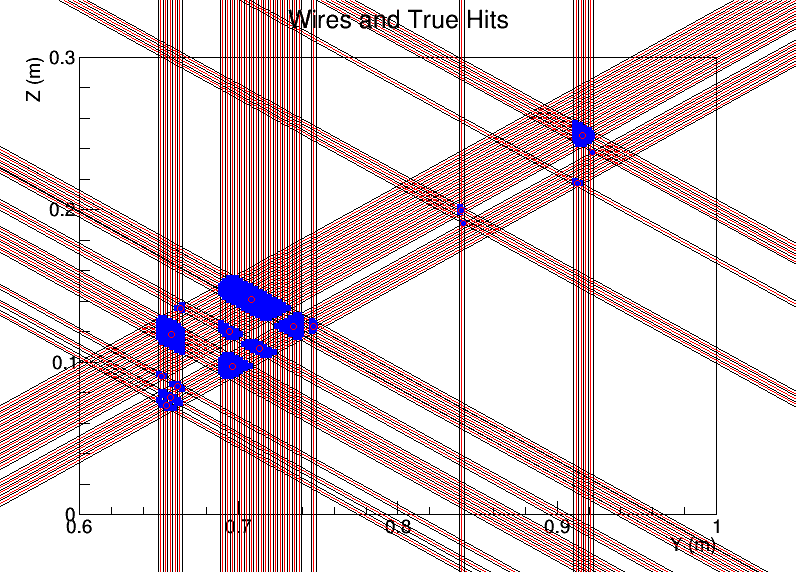
\includegraphics[width=0.8\textwidth]{wires-and-true-hits.png}          
    \end{column}
  \end{columns}
      
  \begin{enumerate}
  \item Select cells with their three wires above threshold.
  \item Partition set into spatially contiguous subsets: ``\textbf{blobs}''.
  \end{enumerate}
  Equation to solve becomes:
  \[\vec{w_b} = \mathbf{G_{wb}} \vec{b}\]

  \begin{description}
  \item[$\vec{b}$] vector of charge in each blob.
  \item[$\mathbf{G_{wb}}$] the wire-blob adjacency matrix for the slice.
  \item[$\vec{w_b}$] vector of charge on all wires associated with a blob.
  \end{description}

  Now, often \textbf{more favorable numerology}: $N_{blob} \lesssim N_{w_b}$
\end{frame}

% maybe remove this slide...
\begin{frame}
  \frametitle{Another wrinkle: charge uncertainty}

  Each wire's measure of drifting charge is uncertain.
  \begin{itemize}
  \item Environmental, electronic and thermal noise.
    \begin{itemize}\footnotesize
    \item[$\rightarrow$] Can be correlated across wires/channels/chips/boards/etc.
    \end{itemize}
  \item Statistical uncertainty due to digitization.
  \item Systematic uncertainties from deconvolution.
  \end{itemize}

  \vspace{3mm}

  Form a $\chi^2$ comparing measured wire charge ($\vec{w}_{meas}$)
  with expected ($\vec{w}_{exp}$) and covariance uncertainty matrix
  $\mathrm{V}$.
  
  \[\chi^2 = (\vec{w}_{meas}-\vec{w}_{exp})^\intercal\mathrm{V}^{-1} (\vec{w}_{meas}-\vec{w}_{exp})\]

  \vspace{3mm}

  \begin{center}
    \textbf{$\rightarrow$ This is a very CPU intensive, but critical step!}
  \end{center}

  \footnotesize And recall:
  \begin{itemize}
  \item this must be done at the raw-data processing stage
  \item need to do this each \SI{2}{\milli\second} time slice
  \end{itemize}

\end{frame}

\begin{frame}[fragile]
  \frametitle{The Payoff: imaged \SI{3}{\giga\electronvolt} $\nu_e$ interaction}
  
  \begin{columns}
    \begin{column}{0.5\textwidth}
      \begin{center}
        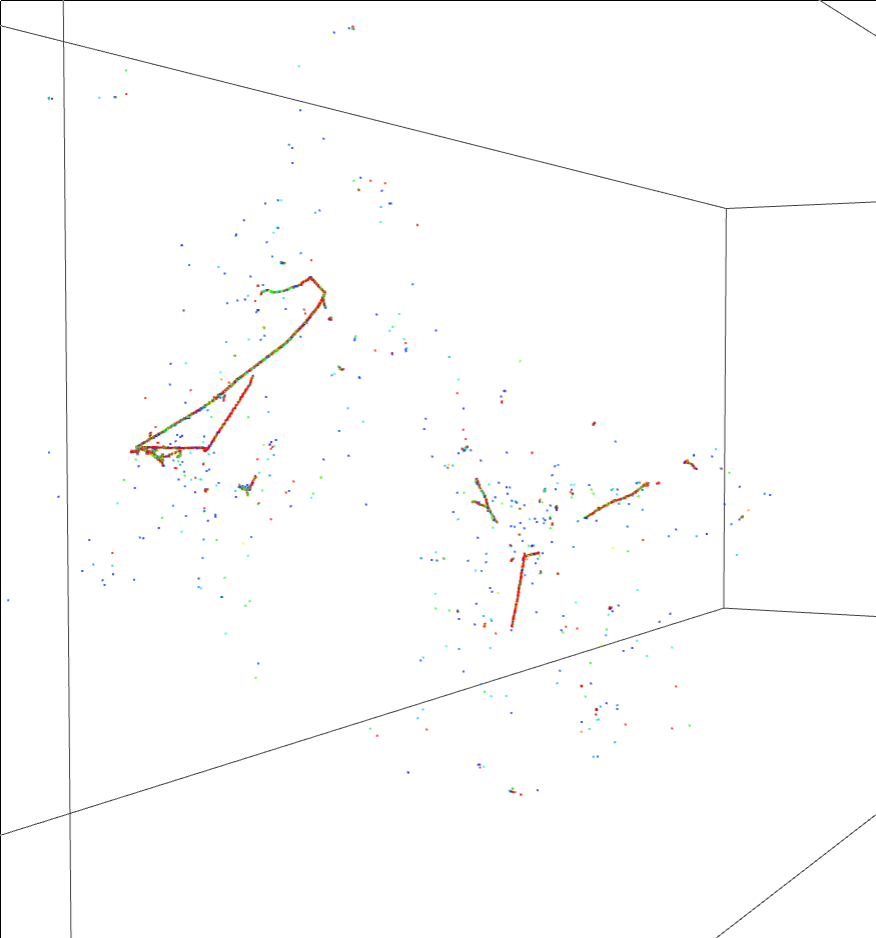
\includegraphics[width=\textwidth,trim=3cm 10cm 3cm 10cm,clip]{payoff-true.png}

        True energy depositions.
      \end{center}
    \end{column}
    \begin{column}{0.5\textwidth}
      \begin{center}
        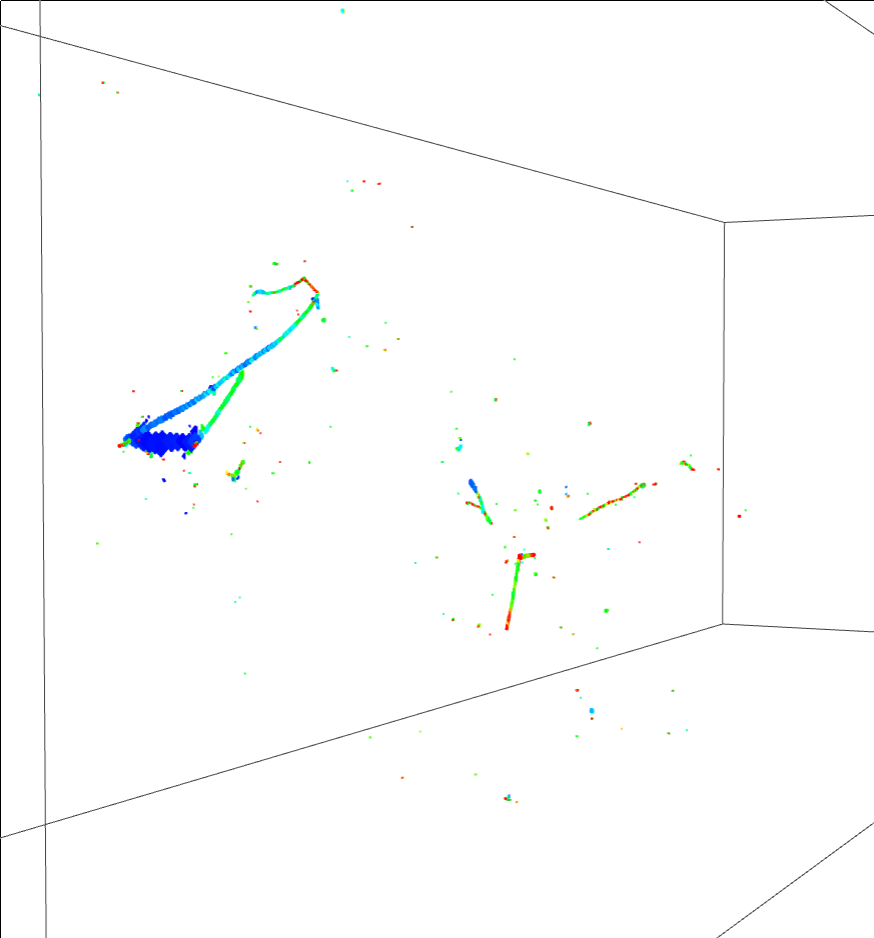
\includegraphics[width=\textwidth,trim=3cm 10cm 3cm 10cm,clip]{payoff-reco.png}

        Wire Cell Imaging.
      \end{center}
    \end{column}
  \end{columns}

  \vfill

  \footnotesize
  \begin{itemize}
  \item \textbf{Excellent imaging} of major track features as well as isolated
    activity.
    \begin{itemize}\scriptsize
    \item[$\rightarrow$] a static 2D view doesn't do it justice!  \href{http://www.phy.bnl.gov/wire-cell/bee/set/6/event/0/}{Follow link to try it}.
    \end{itemize}
  \item \textbf{Residual ambiguity} seen as wide blue patches.
    \begin{itemize}\scriptsize
    \item[$\rightarrow$] \textbf{Inherent in LArTPC technology}, Wire Cell just makes it evident.
      \begin{itemize}\scriptsize
      \item due to activity running parallel to the wire plane in one time slice.
      \end{itemize}
    \item[$\rightarrow$] Pursue
      an \textbf{iterative} approach: constrain ambiguous regions
      after taking well reconstructed parts to the kinematics-level.
    \end{itemize}
  \end{itemize}
\end{frame}


\subsection{Pattern Recognition}

\begin{frame}
  \frametitle{Pattern Recognition}
  Our current \textbf{post-imaging} approach:
  \begin{enumerate}
  \item \textbf{cluster} together blobs contiguous in space and time
    (slice).
  \item \textbf{track} a line through a cluster.
  \item \textbf{categorize} success/failure of track to account for the
    cluster's charge distribution.
  \end{enumerate}
  Some categories:
  \begin{description}
  \item[track] cluster is well characterized by the track.
  \item[shower] cluster consistent with an EM/hadronic shower.
  \item[short] cluster appears to be a ``short track'' (eg, $\delta$-ray).
  \item[undefined] no well-suited categorization.
  \end{description}

  \begin{itemize}
  \item This is an \textbf{active area of development} for Wire Cell.
  \item Maybe a problem suited for \textbf{machine learning}? 
  \end{itemize}

\end{frame}

\section{Wire Cell Software}

\begin{frame}
  \tableofcontents[currentsection,hideothersubsections]
\end{frame}


\begin{frame}
  \frametitle{Wire Cell Software Ecosystem}

  The software is composed into three main parts:

  \vspace{3mm}

  \begin{description}
  \item[visualization] the ``Bee'' web application (Chao Zhang)
  \item[prototype] reconstruction algorithms, initial proof of
    principle (Xin Qian)
  \item[toolkit] production process, parallelism and basis for long-term development (bv)
  \end{description}

\end{frame}

\subsection{Bee Display}

\begin{frame}
  \frametitle{Bee: an interactive 3D visualization system}

  Select features:
  \begin{itemize}
  \item \textbf{Web browser-based} 3D event display, 
  \item Shows variety of reconstructed and ``true'' information.
  \item Implemented in \textbf{JavaScript/WebGL} (\textbf{Django} backend).
  \item Simple \textbf{JSON} data file format, 
    \begin{itemize}
    \item \href{http://bnlif.github.io/wire-cell-docs/viz/uploads/}{drag-and-drop user
      file uploads}.
    \end{itemize}
  \end{itemize}

  \onslide<2->{ 
    \textbf{Bee 2.0} in development
    \begin{itemize}
    \item[$\rightarrow$] \textbf{semi-automated, human-guided} pattern
      recognition.
    \item[$\rightarrow$] collect and replay human decisions.
    \item[$\rightarrow$] look for \textbf{low-hanging fruit to
        automate}.
    \item[$\rightarrow$] maybe feed into machine learning?
    \end{itemize}}

\end{frame}

\begin{frame}
  \frametitle{Bee Screenshot}
  \begin{center}
    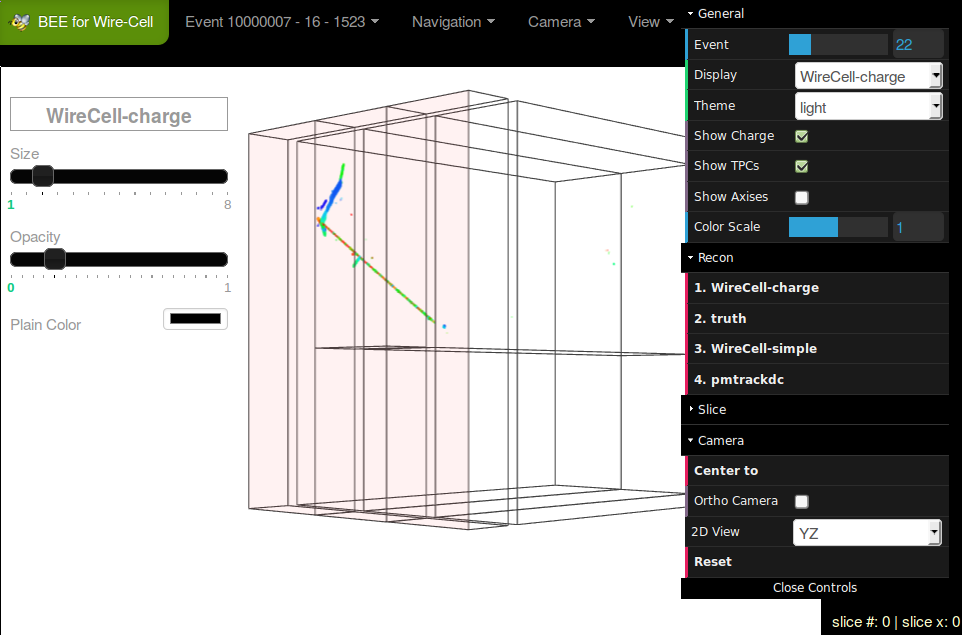
\includegraphics[height=0.7\textheight]{bee-full-gui.png}    
  \end{center}
  \begin{center}
    Try it yourself: \url{http://www.phy.bnl.gov/wire-cell/bee/}
  \end{center}
\end{frame}


\subsection{Prototype}

\begin{frame}
  \frametitle{Wire Cell Working Prototype}
  \footnotesize

  \begin{itemize}
  \item \textbf{Very successful proof of principle!}
  \item Currently \textbf{leads the state of the art} in LArTPC
    reconstruction techniques.
  \end{itemize}

  \begin{center}
    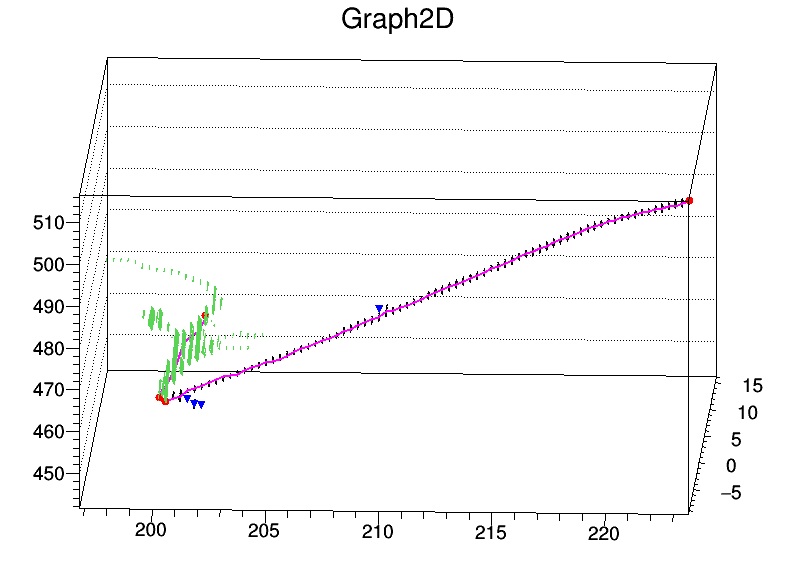
\includegraphics[height=0.5\textheight,trim=0cm 0cm 0cm 2cm,clip]{xin-shower.png}

    \scriptsize
    Example result showing imaging + pattern recognition.  Colors indicate identified tracks and showers.
  \end{center}

\end{frame}

\subsection{Toolkit}

\begin{frame}
  \frametitle{Wire Cell Toolkit}

  \begin{columns}
    \begin{column}{0.65\paperwidth}
    \end{column}
    \begin{column}{0.35\paperwidth}
      \vspace{-20mm}
      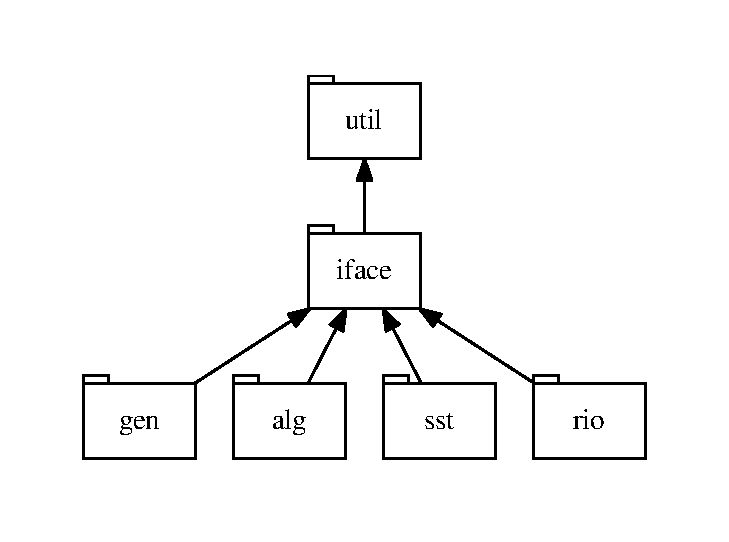
\includegraphics[width=\textwidth]{deps.pdf}      
    \end{column}
  \end{columns}

  \vspace{-15mm}

  Address compromises made in the name\\
  of rapid prototyping 
  \begin{itemize}
  \item Modular \textbf{packaging and build} system (waf).
  \item Comprehensive \textbf{API} via abstract interface classes.
  \item Mindful of \textbf{dependencies}, external and internal.
  \item Built-in wire and cell \textbf{geometry descriptions} or load from file.
  \item Includes simple \textbf{LArTPC detector simulation}.
  \item Rewriten implementations of \textbf{prototype algorithms}.
  \item \textbf{Data Flow Programming} execution model with \textbf{abstracted DFP engine}.
  \end{itemize}

  \vfill

  Just now becoming available but with some work still to do.

\end{frame}

\begin{frame}[fragile]
  \frametitle{Wire Cell Execution Model}

  \begin{columns}
    \begin{column}{0.7\textwidth}
      \footnotesize 
      The toolkit supports \textbf{data flow programming} paradigm
      \begin{itemize}
        \item Design influenced by
          \href{http://www0.bnl.gov/events/details.php?q=8932}{VisTrails} and others.
        \item Data flows through a \textbf{graph} made from:
          \begin{description}
          \item[vertices:] \textbf{computational units} (algorithms)
          \item[edges:] \textbf{data queues} of a given type
          \end{description}
        \item Streamed processing minimizes RAM usage.
        \item High-level ``graph programming'' in user config.
        \item \textbf{Thread-safe queues $\Rightarrow$ parallel processing.}
        \item Abstract graph execution machinery.
          \begin{itemize}\scriptsize
          \item Intel TBB provides reference implementation.
          \end{itemize}
        \end{itemize}
      \end{column}
      \begin{column}{0.3\textwidth}

        \vspace{-10mm}

        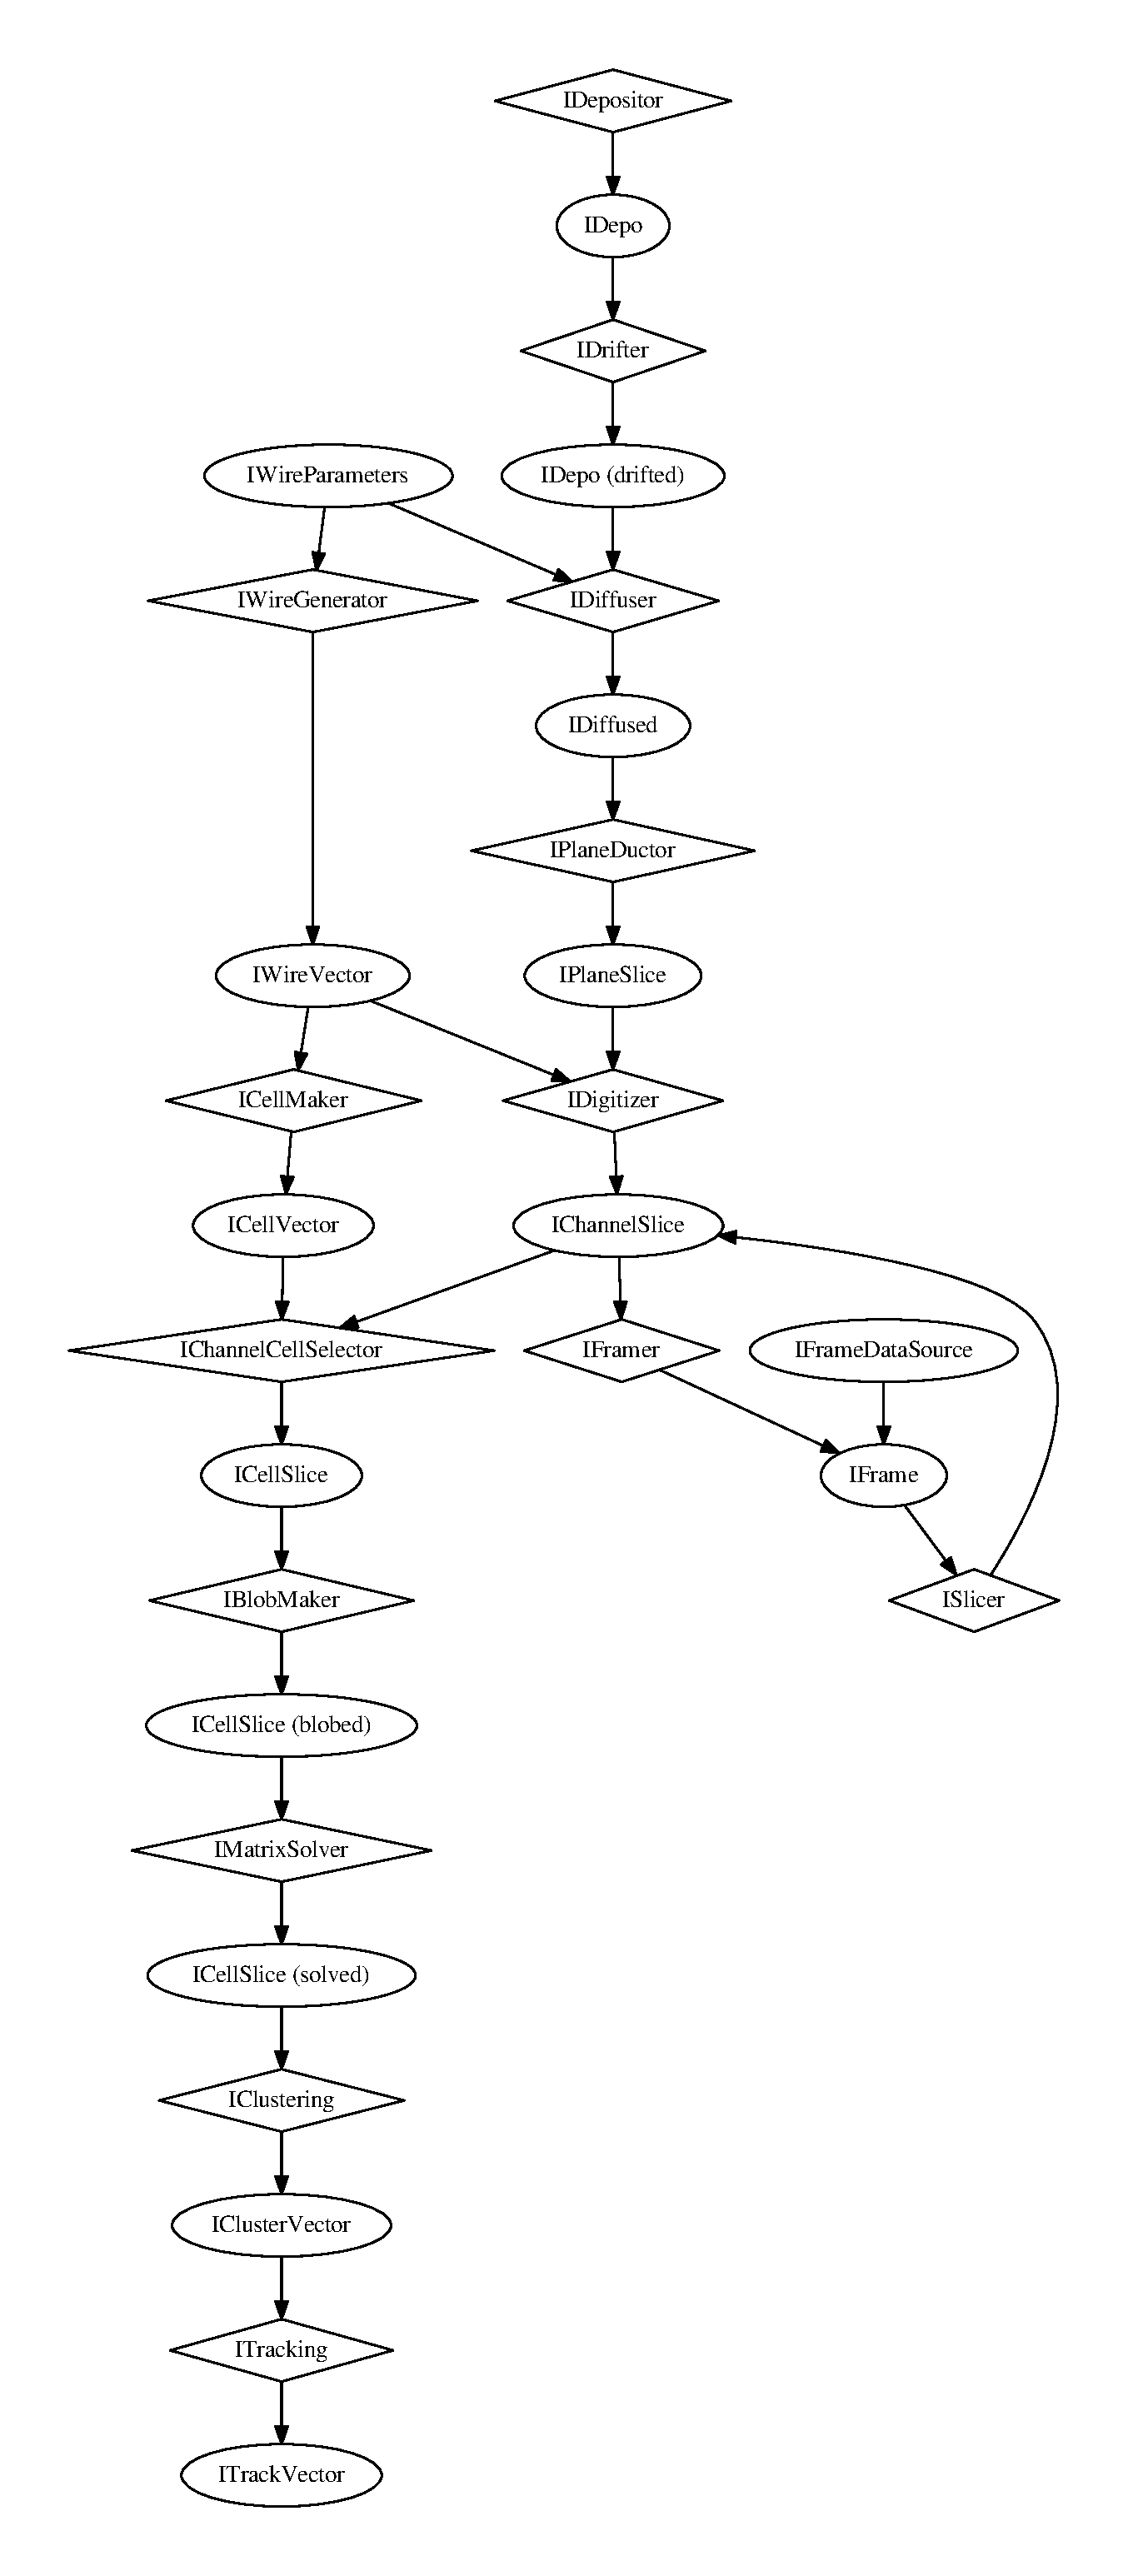
\includegraphics[width=\textwidth]{dataflow.pdf}

        \tiny One possible Wire Cell flow.
      \end{column}
    \end{columns}
\end{frame}




\section{}

\begin{frame}
  \frametitle{Summary}
  \footnotesize
  \begin{itemize}
  \item The \textbf{Wire Cell working prototype LArTPC reconstruction} method and software has been developed.
    \begin{itemize}  \footnotesize
    \item already producing some of the \textbf{world's best results},
    \item technical and performance improvements on-going.
    \end{itemize}
  \item The \textbf{Bee interactive 3D event visualization}
    application developed, critical for understanding LArTPC and
    developing Wire Cell.  Plans to evolve to ``human-directed
    automated reconstruction'' system.
  \item The \textbf{Wire Cell Toolkit} for LArTPC reconstruction
    partly complete and will be the basis for long term development
    including investigations into parallel processing.
  \item To be successful we must wade into \textbf{new waters} (for
    us) of parallel processing, hardware acceleration, computing
    science and mathematics.
  \end{itemize}

  \begin{center}
    $\rightarrow$ \textbf{Expert input, help and collaboration are
      most welcome!}
  \end{center}
\end{frame}

\begin{frame}
  \frametitle{Wire Cell on the web}

  \begin{itemize}
  \item home page: \\ \url{http://www.phy.bnl.gov/wire-cell/}
  \item Bee entry page: \\ \url{http://www.phy.bnl.gov/wire-cell/bee/}
  \item prototype user manual: \\ \url{http://bnlif.github.io/wire-cell-docs/}
  \item prototype repositories: \\ \url{https://github.com/BNLIF}
  \item toolkit user manual: \\ \url{http://wirecell.github.io/wire-cell-docs/}
  \item toolkit code reference: \\ \url{http://www.phy.bnl.gov/wire-cell/doxy/html/}
  \item toolkit repositories: \\ \url{https://github.com/WireCell}
  \end{itemize}
\end{frame}


\end{document}


%%% Local Variables:
%%% mode: latex
%%% TeX-master: t
%%% End:
